\documentclass[dvisvgm,tikz,border=4pt]{standalone}\usepackage{amsmath,amssymb}
\usetikzlibrary{arrows.meta,decorations.markings,backgrounds,cd,calc}
\colorlet{c1}{blue!70!black}\colorlet{c2}{red!70!black}\colorlet{c3}{green!45!black}
\tikzset{
 ->-/.style={decoration={markings,mark=at position .55 with {\arrow{Stealth[length=2.4mm]}}},postaction={decorate}},
 ->>-/.style={decoration={markings,mark=at position .5 with {\arrow{Stealth[length=2.4mm]}},mark=at position .6 with {\arrow{Stealth[length=2.4mm]}}},postaction={decorate}},
 every picture/.append style={show background rectangle, background rectangle/.style={fill=white}}
}

\begin{document}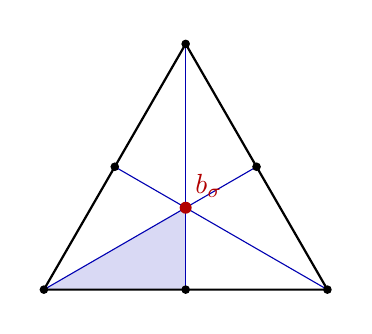
\begin{tikzpicture}[scale=1.2]
\coordinate (A) at (0,0); \coordinate (B) at (3,0); \coordinate (C) at (1.5,2.6);
\coordinate (O) at (1.5,0.8667); \coordinate (AB) at (1.5,0); \coordinate (BC) at (2.25,1.3); \coordinate (AC) at (0.75,1.3);
\fill[c1!15] (A)--(AB)--(O)--cycle;
\draw[thick] (A)--(B)--(C)--cycle;
\foreach \p in {A,B,C,AB,BC,AC} \draw[c1] (O)--(\p);
\foreach \p in {A,B,C,AB,BC,AC} \fill (\p) circle(1.3pt);
\fill[c2] (O) circle(1.8pt) node[above right,c2]{$b_\sigma$};
\end{tikzpicture}\end{document}
